% #############################################################################
% This is Chapter 6
% !TEX root = ../main.tex
% #############################################################################
% Change the Name of the Chapter i the following line
\fancychapter{User Studies}
%\cleardoublepage
% The following line allows to ref this chapter
\label{chap:UserStudies}
To evaluate the developed Trust Model we conducted a user study using the Quick Numbers scenario  (Figure \ref{fig:ParticipantQuickNumbers}) previously described in Chapter \ref{chap:Scenario}, and \ac{EMYS} (Figure \ref{fig:EMYS}) as the robot to embody the virtual agent. Additionally, the user study was also executed in conjunction with Henriques to test his own Rapport model. The study was performed in a between subjects design, focusing on checking if Trust would increase between conditions where the model's Action Suggestion component is either active or inactive. Trust is measured through a questionnaire, later described in Section \ref{sec:MethodologyAndProcedures}, and also with the Investment scenario value. The scenario was implemented in a touch-screen table, with the Unity Engine.

\begin{figure}[h]
    \centering
    \begin{minipage}[b]{.60\textwidth}
        \centering
        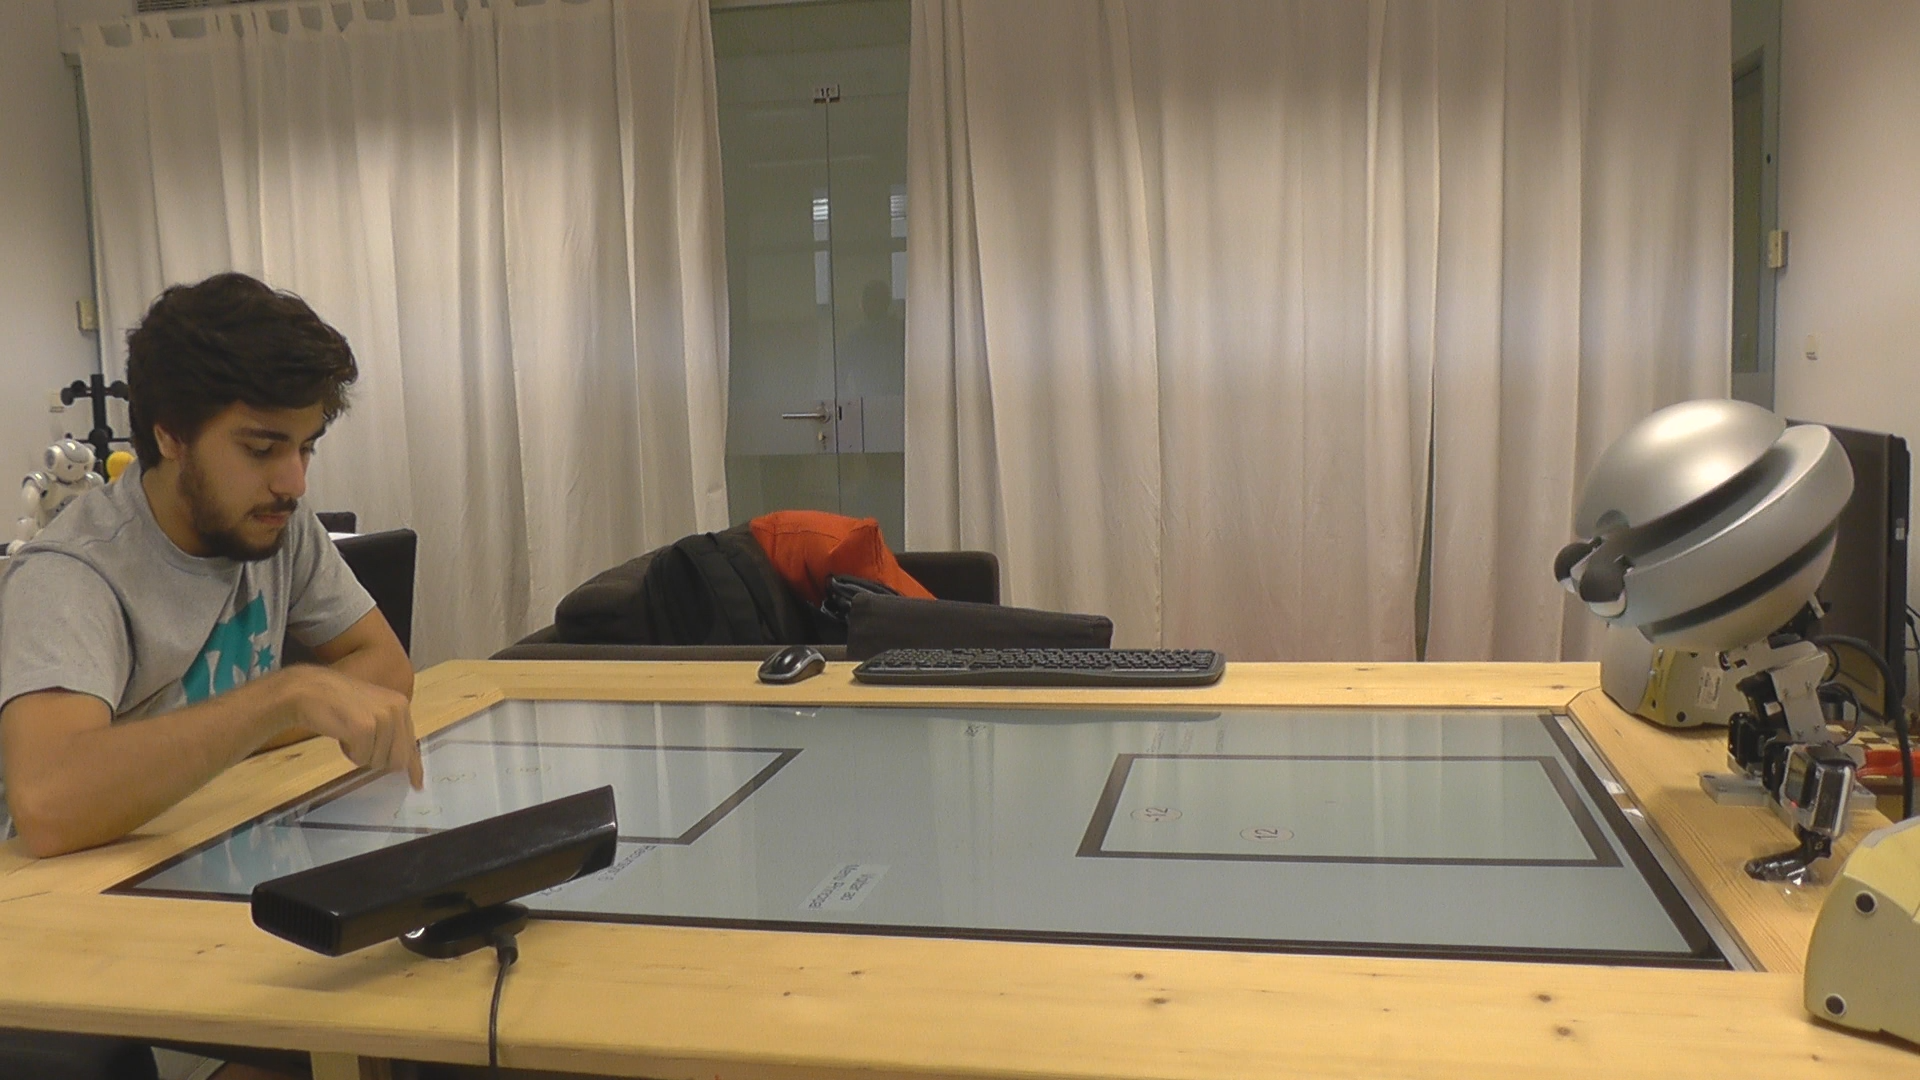
\includegraphics[width=\textwidth]{figures/ScenarioScreenShot.png}
        \caption{Participant playing with \ac{EMYS} in the Quick Numbers scenario}
        \label{fig:ParticipantQuickNumbers}
    \end{minipage}
    \hfill
    \begin{minipage}[b]{.30\textwidth}
        \centering
        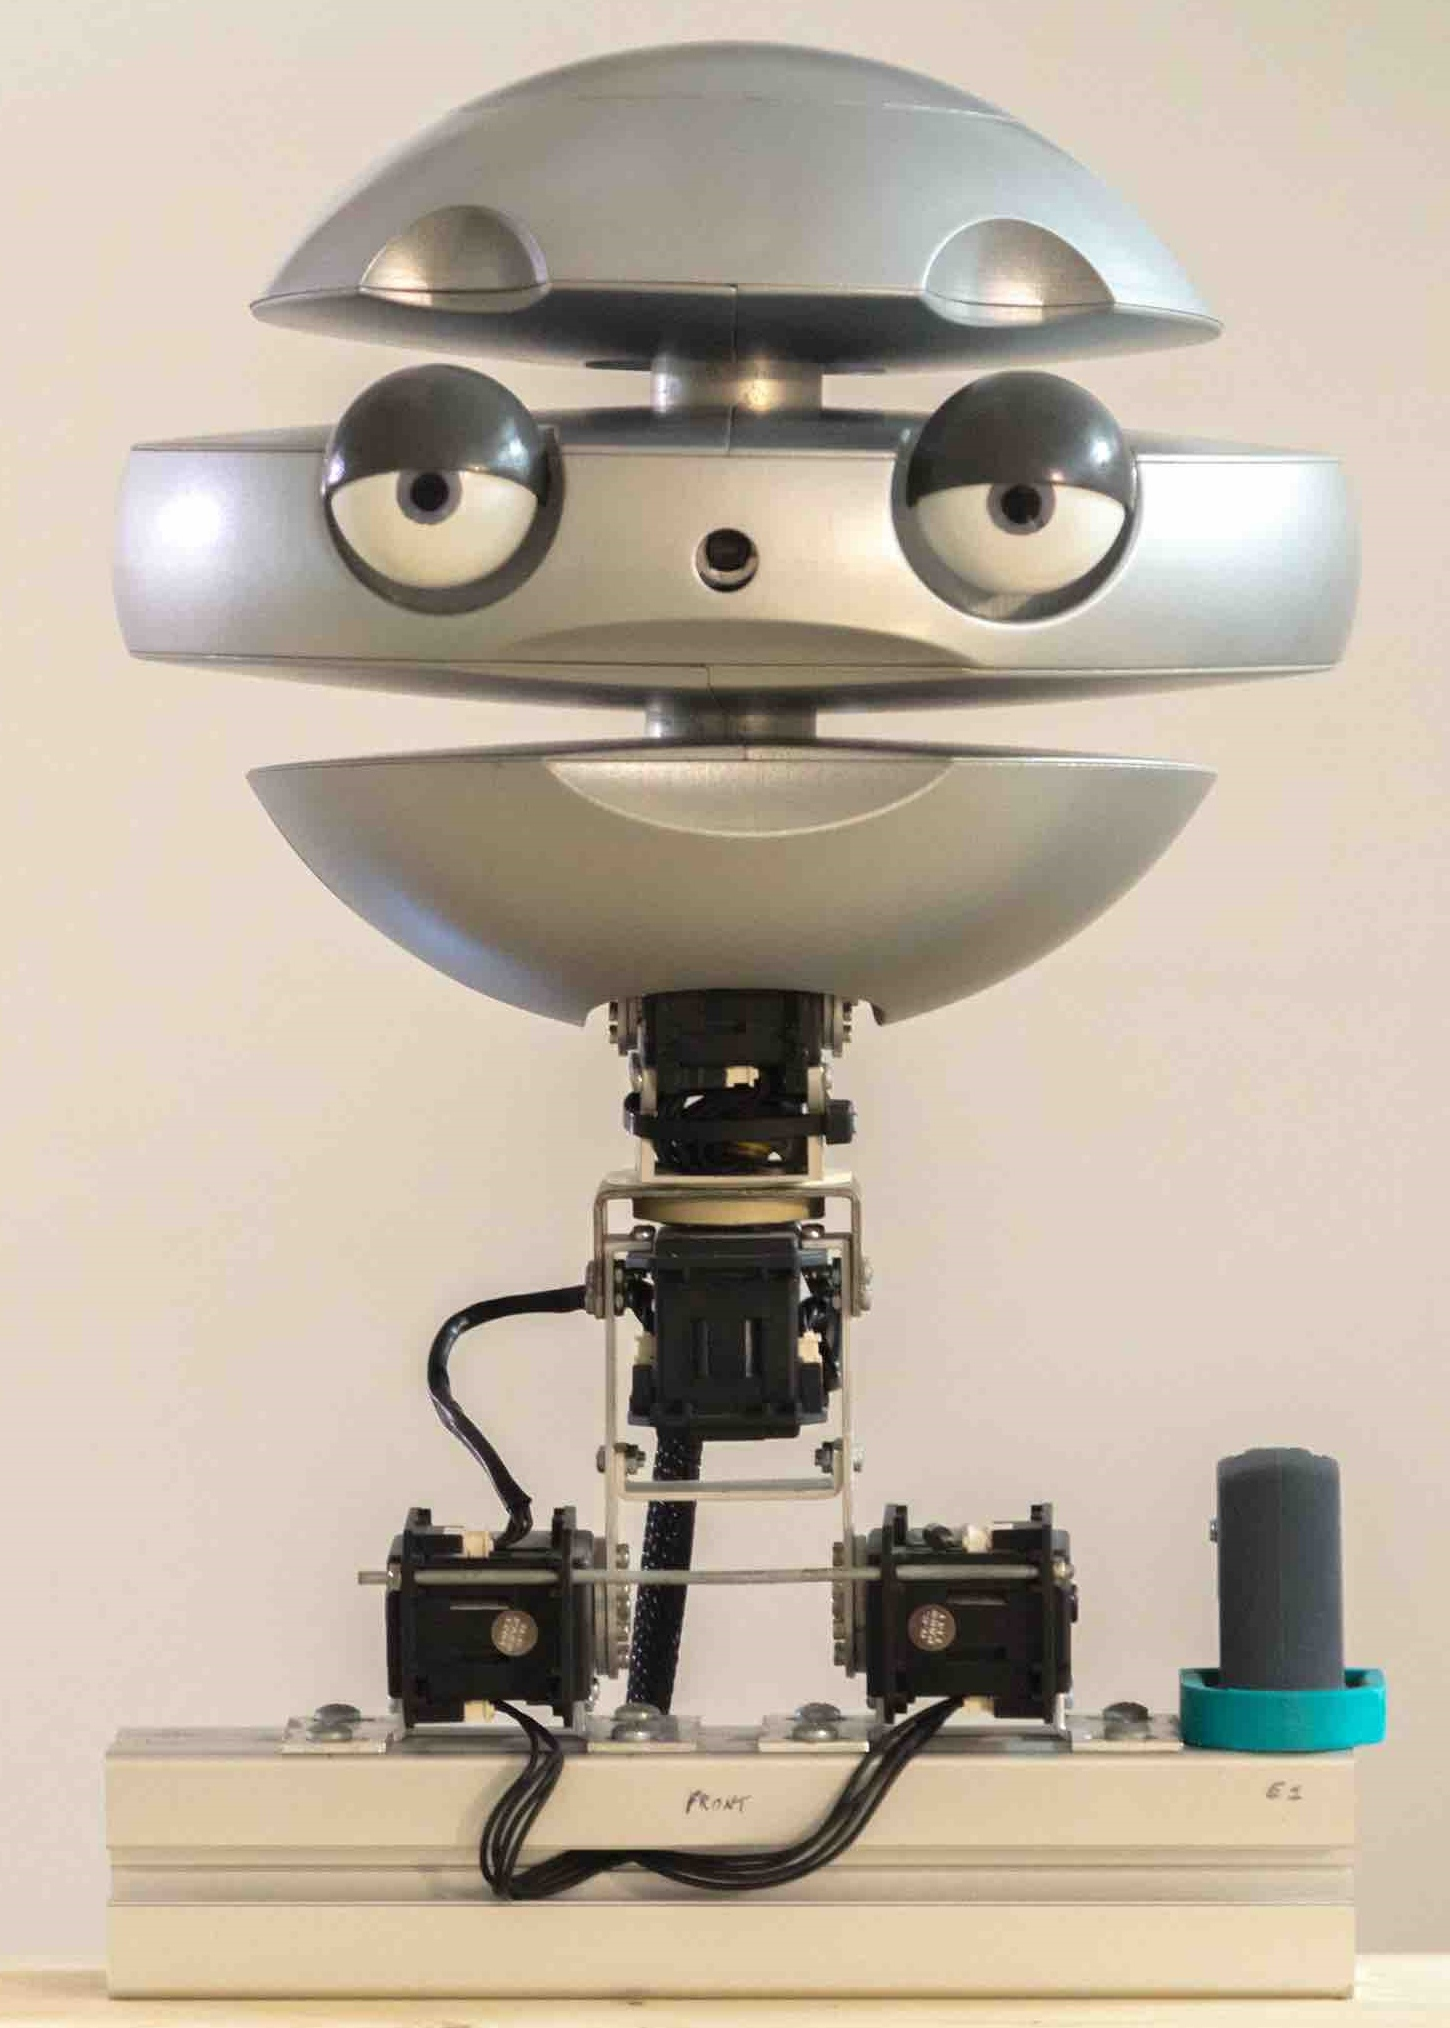
\includegraphics[width=\textwidth]{figures/emys.jpg}
        \caption{\ac{EMYS} Robot}
        \label{fig:EMYS}
    \end{minipage}
\end{figure}

\section{Scenario and Game Parametrization}
The scenario was designed with a series of parameters, mainly for the game and AI, that were defined for the User Studies, as seen in Table \ref{tbl:ScenarioConfigurations} and Figure \ref{fig:ScenarioConfigs}.

\begin{table}[h]
    \centering
    \begin{tabular}{|l|l|}
        \hline
        \textbf{Parameter}              &  \textbf{Value}   \\ \hline
        \multicolumn{2}{|l|}{\textbf{Scenario}}             \\ \hline
        $Starting\ Resources$           &  10               \\ \hline
        \multicolumn{2}{|l|}{\textbf{Game}}                 \\ \hline
        $Starting\ Multiplier$          &  0.0x             \\ \hline
        $Time\ For\ Game$               &  30 seconds       \\ \hline
        $Target\ Spawn\ Interval$       &  0.5 seconds      \\ \hline
        $Chance\ For\ Wrong\ Target$    &  70\%             \\ \hline
        $Positive\ Ratio$               &  60\%             \\ \hline
        $Target\ Lifetime$              &  2.7 seconds      \\ \hline
        $Gain\ Per\ Correct\ Target$    &  0.2x             \\ \hline
        $Loss\ Per\ Wrong\ Target$      &  -0.1x            \\ \hline
        \multicolumn{2}{|l|}{\textbf{Game's AI}}            \\ \hline
        $Clicking\ Interval\ (C_i)$     &  0.5 seconds      \\ \hline
        $Reaction\ Time\ (R_t)$         &  0.3 seconds      \\ \hline
        $Chance\ of\ Right\ Target\ (C_r)$ & 70\%           \\ \hline
    \end{tabular}
    \caption{Scenario Configurations}
    \label{tbl:ScenarioConfigurations}
\end{table}

\begin{figure}[hbt]
    \centering
    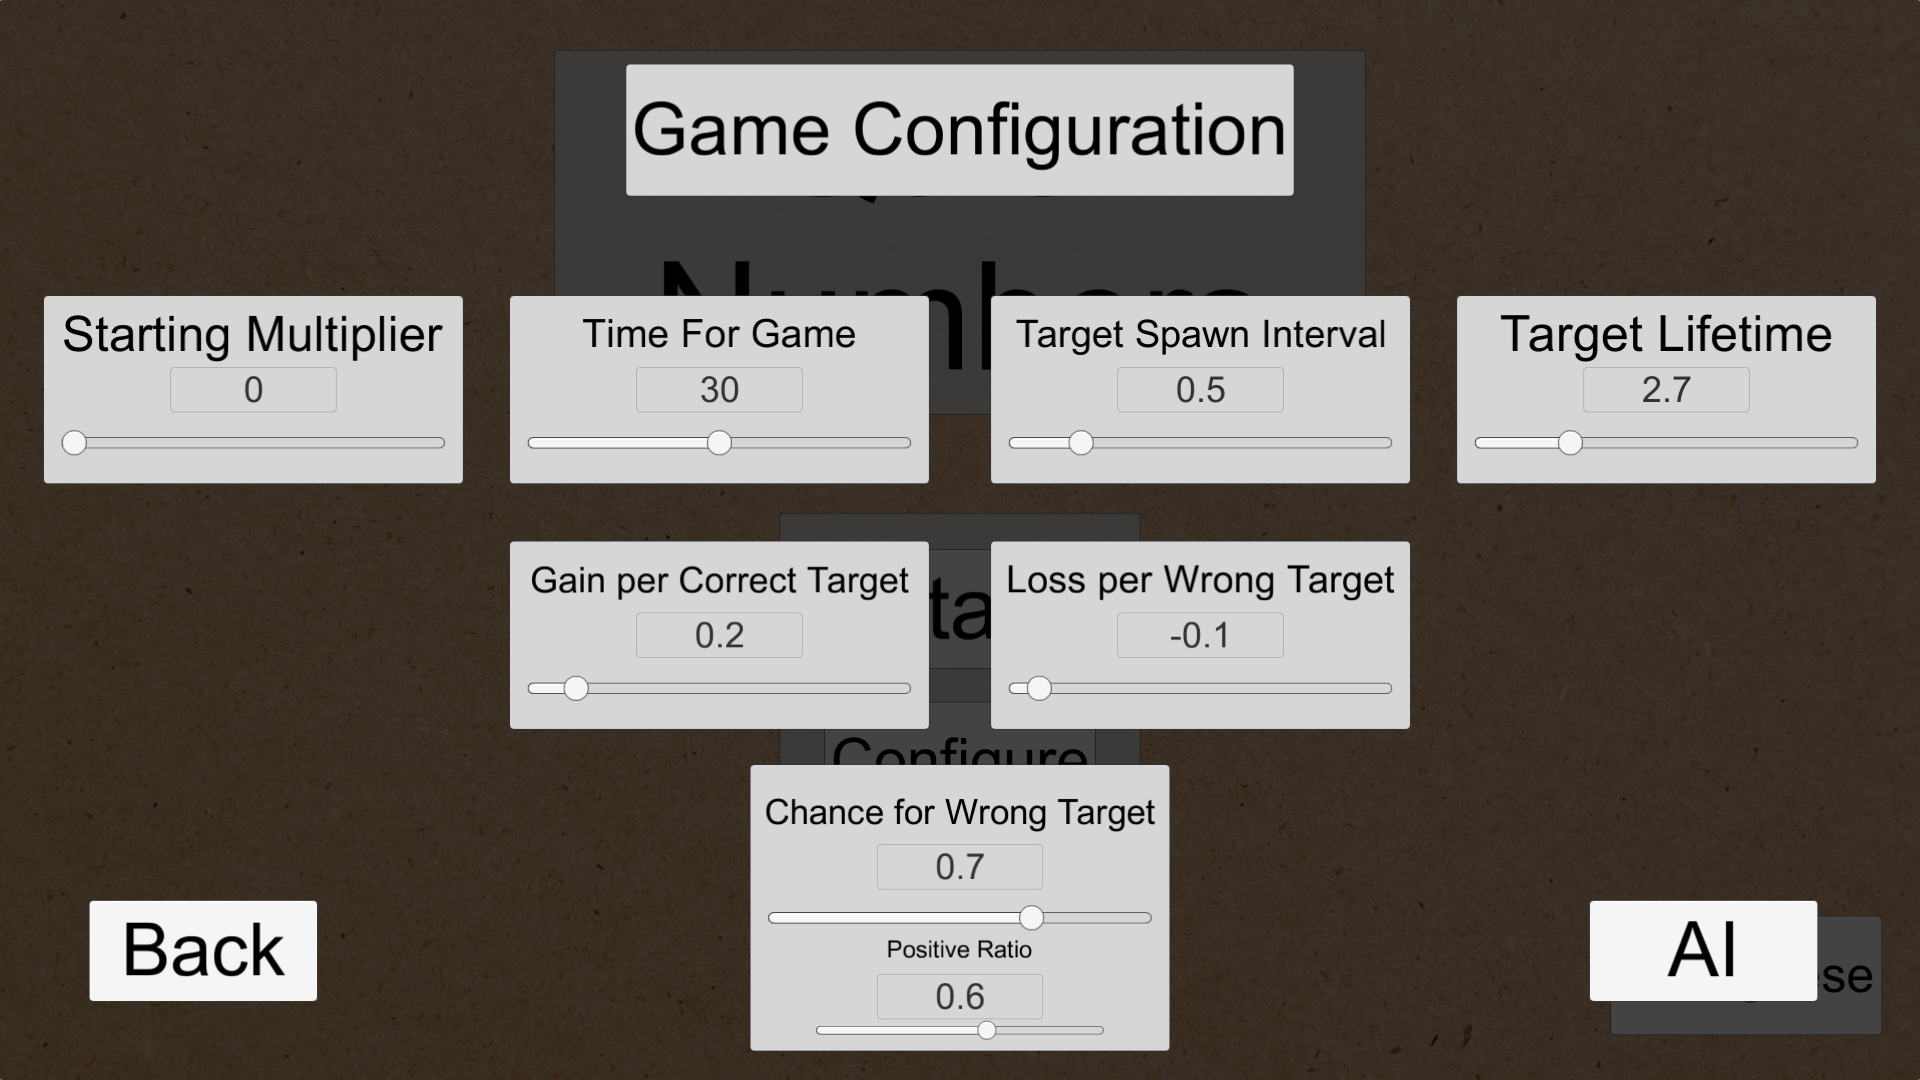
\includegraphics[width=0.8\textwidth]{figures/GameConfigs.png}
    \caption{Screenshot of Scenario Configurations Editor}
    \label{fig:ScenarioConfigs}
\end{figure}

Regarding the \ac{AI} parameters: we wanted the agent to play rapidly, if a little recklessly, as to provide more opportunities for the participant to react and notice how he played, so we empirically found 0.5 seconds to be a good value for $C_i$, as it made the agent have a slightly above average human reaction time for pressing the circles. To $C_r$ we assigned 70\% success rate, as failing 30\% of the circles averaged out the agent's score to normal human achievable levels, and to $R_t$ we selected 0.3 seconds, as it is plausible value for a 30\% fail chance, as the agent simulates not entirely recognizing the number before pressing the circle.


\section{Agent Architecture}
The agent we used to serve as a host to the Trust Model was built using Henriques' Rapport Controller \cite{Henriques2016}, a computational framework developed to create human agent interactions and transmit them to the various components that control the agent embodiment. This version of the framework is built upon \ac{SERA}'s ecosystem \cite{Ribeiro2003}, an architectural model that gathers and connects a series of tools to control a robotic embodiment, namely:

\begin{itemize}
    \item \textbf{Thalamus}: A networking module that enables the exchange of actions and perceptions between the various agent's modules. All communication coming from the controller to the robot actuators and scenario sensors come through this module;
    \item \textbf{Skene}: A behaviour planner that translates high-level intentions to actions. For the purpose of the Rapport Controller the main use of Skene is to perform animation planning, lip-syncing and handling gaze. Additionally, it provides simple way to input these intentions, through a simple markup language.
    \item \textbf{Nutty Tracks}: An animation engine that performs the animations of the embodied agent;
    \item \textbf{Speech Server}: A simple \ac{TTS} server to perform utterances.
\end{itemize}
              
The Rapport Controller uses a plug-in architecture, with the controller itself serving only as platform of communication between the behaviour plug-ins, where the user may load and unload plug-ins on-the-fly. One of this plug-ins, Agent Actions Manager, is integrated into the controller, as it serves as a wrapper interface to communicate with the SERA environment. It is specially important for our agent implementation, as it provides a convenient way to propose utterances and animations to the agent, by allowing the import of a text .csv data file in a table format exemplified in Table \ref{tbl:UtteranceDataFormat} and with the following field descriptions:

\begin{itemize}
    \item \textbf{Category}: This field serves as a sort of namespace to identify the utterance;
    \item \textbf{Subcategory}: The pair Category - Subcategory identifies the utterance. If 2 or more utterances have the same pair, one of them is randomly chosen to be proposed when called;
    \item \textbf{Utterance}: This field represents an utterance to be performed by the agent. Elements between \textless...\textgreater\ are animation cues, which are synchronised and proposed to the Agent. And \textbar...\textbar\ are substitution keys, that enable proposing utterances with variables;
    \item \textbf{Priority}: If 2 or more utterances are in conflict to be performed by the agent, the one with higher priority will take over and be performed;
    \item \textbf{Delay (ms)}: Defines a time to wait before starting the utterance;
    \item \textbf{Timeout (ms)}: If the utterance performance is taking longer than the value defined in this field, it is prematurely ended. 
\end{itemize}

Along the scenario, the agent will perform some simple interaction utterances, depending on the scenario phase and state. We used slightly different tables for utterances for each condition, as the table for condition B includes the utterances used by the Actions in the model. The utterance tables can be seen in Appendix \ref{app:UserStudiesQuestionnaire}.

\begin{table}[h]
\centering
\begin{tabular}{|l|l|l|l|l|l|}
    \hline
    \textbf{Category}   & \textbf{Subcategory}  & \textbf{Utterance} & \textbf{Priority} & \textbf{Delay(ms)} & \textbf{Timeout (ms)}\\ \hline
    session             & start                 & Hi, \textless Gaze(middleFront)\textgreater I'm Emys! & 2 & 0 & 2000 \\ \hline
    match               & end                   & I've won \textbar\textit{quantity}\textbar\ resources. & 2 & 0 & 2000 \\ \hline
    
    
\end{tabular}
\caption{Examples of Utterance Data Format.}
\label{tbl:UtteranceDataFormat}
\end{table}

Three main plug-ins were developed for the Rapport Controller:
\begin{itemize}
    \item \textbf{Scenario Perceiver}: serves as a notifier to the other plug-ins about changes in the environment.
    \item \textbf{Scenario Script}: enables the Agent to progress through the scenario by performing scripted behaviours that are triggered by notifications from the Scenario Perceiver. This includes the choice of how much it invests on the game it plays, which is always half of the resources it has at the time. How much it returns to the participant in the last stage is also scripted, the amount returned being the participant's investment multiplied by the agent's multiplier score in the respective game (e.g. If 10 was invested and the agent scores a multiplier of 2.4x, it returns 24 resources).
    \item \textbf{Trust Model}: an implementation of trust model described in Chapter \ref{chap:TrustModel}, albeit with some alterations further explained in Section \ref{subsec:TrustModelPlugin}.
\end{itemize}

\subsection{Trust Model Plug-in}
\label{subsec:TrustModelPlugin}
The Trust Model was implemented as a plug-in to the Rapport Controller. Although most of the model is implemented as described in Chapter \ref{chap:TrustModel}, there were some simplifications made to the model:

\begin{itemize}
    \item Trust Calculation described in Section \ref{subsec:TrustCalculation} does not include the $D^j_{F_i}$ parameter, as the amount of time that passes in the scenario is negligible;
    \item Action Suggestion lacks Action sorting and selection as described in Section \ref{sec:ActionSuggestion}. Instead only one action is ever associated to an Environment Input, but performing only if the current Trust Value is lower than constant associated to the Action;
    \item Perceptions do not receive the agents as input. Each Perception contains the Trustor and Trustee agents affected in the interaction perceived;
    \item Certainty values were inserted at the identity value of 1.0f, therefore having no effect in model calculation.
\end{itemize} 

\subsubsection{Scenario Ontology}
As described in Section \ref{sec:Scenario Ontology}, an ontology was required for this scenario. A representation of the ontology created can be seen in Figure \ref{fig:ScenarioOntology}.

\begin{figure}[hbt]
    \centering
    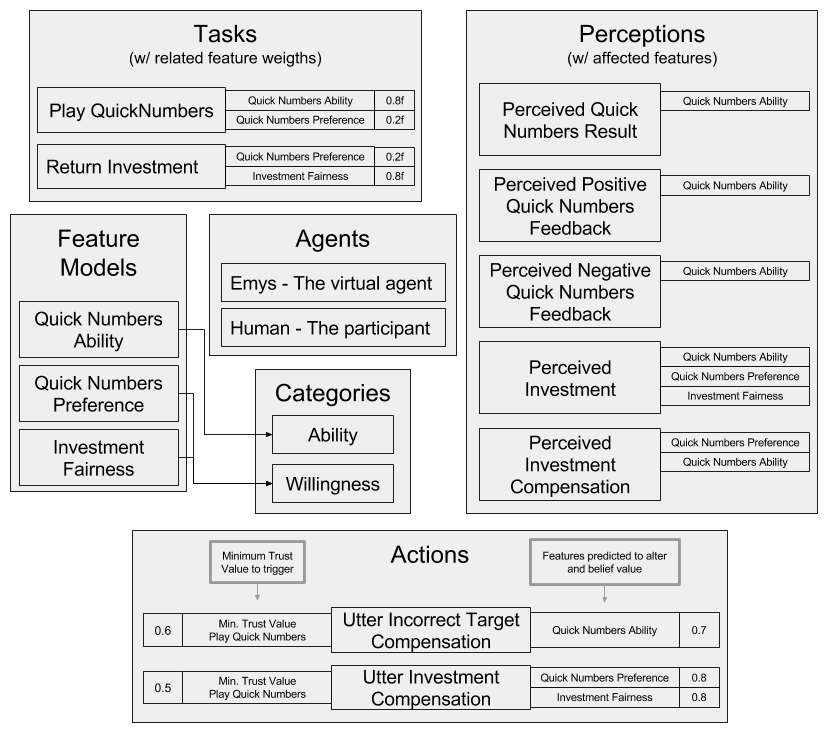
\includegraphics[width=0.9\textwidth]{figures/ScenarioOntology.png}
    \caption{Scenario Ontology}
    \label{fig:ScenarioOntology}
\end{figure}

The utterances performed by the model's action (in Portuguese), and when they are triggered are shown in Table \ref{tbl:TrustModelActionUtterances}.

\begin{table}[h]
    \centering
    \begin{tabular}{|L{0.25\textwidth}|L{0.25\textwidth}|L{0.4\textwidth}|}
        \hline
        \textbf{Action}                         & \textbf{Trigger}                                  & \textbf{Utterance}    \\ \hline
        Utter Incorrect Target Compensation     & Emys Presses Incorrect Target during game         & \textless Animate(sad1)\textgreater\ Hoje a mesa não está a colaborar comigo             \\ \hline
        Utter Investment Compensation           & When participant is choosing the value to invest  & Não tenhas medo de investir! Garanto que consigo multiplicar os recursos. \\ \hline
        
    \end{tabular}
    \caption{Trust Model Action Utterances}
    \label{tbl:TrustModelActionUtterances}
\end{table}

\section{Methodology and Procedures}
\label{sec:MethodologyAndProcedures}
The study was conducted with a between subject design with the following conditions:
\begin{itemize}
    \item \textbf{Condition B}: a baseline condition, where the Action Suggestion component is not active. The data gathered in this condition will serve as the basis to which we compare our results;
    \item \textbf{Condition T}: the condition where Action Suggestion is active, serving as the main results condition.
    \item \textbf{Condition R}: a condition using Henriques' Rapport Model;
    \item \textbf{Condition T+R}: a condition using both ours Action Suggestion component and Henriques' Rapport Model.
\end{itemize}

The conditions R and T+R go out of the scope of this thesis and will not be addressed in this document.

The user study sessions were individual and performed in an closed room accompanied just by the researcher, and lasted between 20 and 30 minutes. The sessions followed the stages as described in Section \ref{sub:stages}, with the interactions performed through the agent and a touch-screen table. Additionally the participants answered a questionnaire, attached in Appendix \ref{app:UserStudiesQuestionnaire}, which is divided in 3 parts, to be filled in different stages of the scenario: 

\begin{itemize}
    \item The first part gathers demographic and sampling information, like gender, age and if the participant had previous interactions with \ac{EMYS}. It also evaluates a participant's self-trust and inclination to trust in others, through a series of questions created by Carrington \cite{Carrington2007}. Participants were asked to fill this before starting the scenario.
    \item The second part is composed of a simple question to self-evaluate trust in the agent, and the trust perception scale described in Section \ref{sec:Related work:The Perception and Measurement of Human-Robot Trust}. This Section was asked to filled at the end of the Investment Stage, immediately after the participant invested on \ac{EMYS}. In fact this serves as the other task that the participant must be doing while the agent plays the game alone.
    \item The third and final part gathers the participant's perception of the agent's Anthropomorphism, Animacy, Likeability and Perceived Intelligence, through the GodSpeed questionnaire \cite{Bartneck2009,Lehmann2015}. It also contains a proximity question by Aron et. al. \cite{Aron1992}. This part was filled by participants at the end of the scenario.
\end{itemize}

The participants were filmed with 2 cameras, with one providing a side-shot of the scene (Figure \ref{fig:ParticipantQuickNumbers}), and the other giving a front-side shot of the participant, from \ac{EMYS} point of view (Figure \ref{fig:ScenarioFrontShot}).

\begin{figure}[hbt]
    \centering
    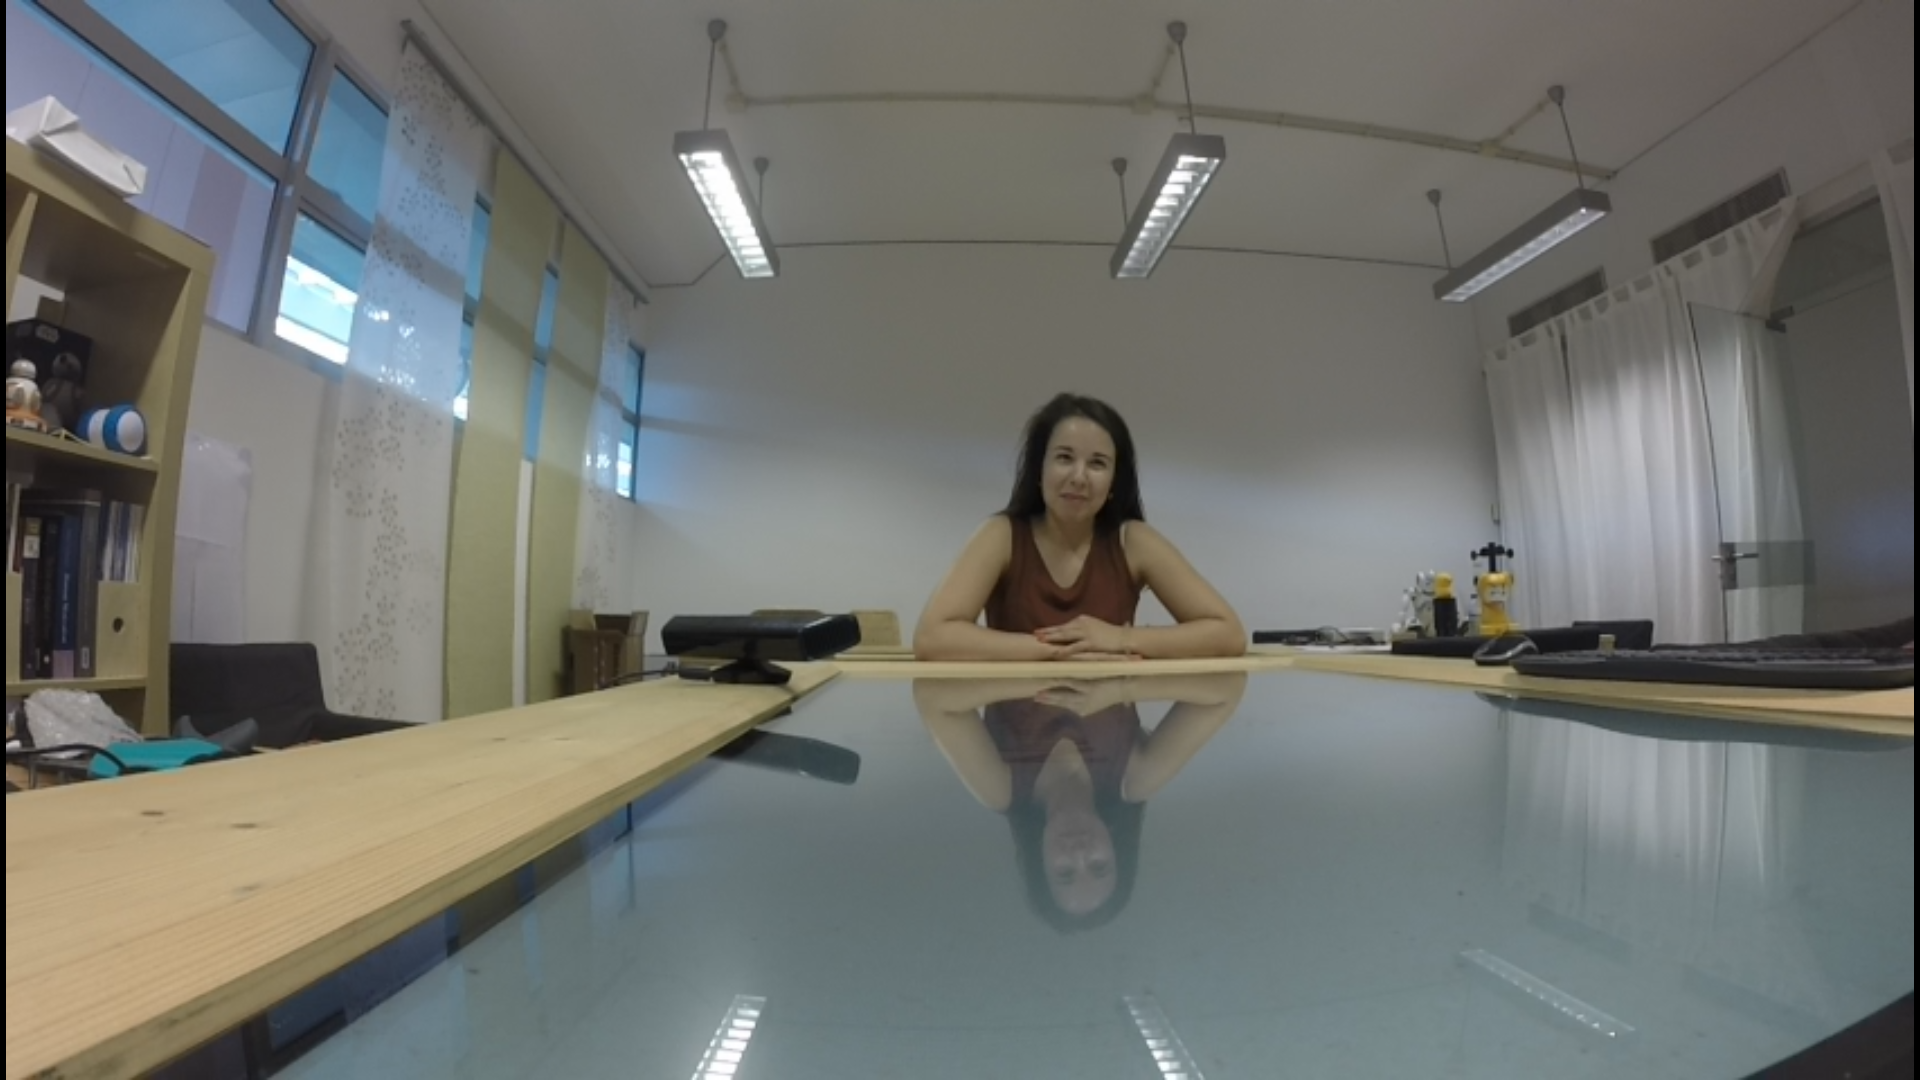
\includegraphics[width=0.4\textwidth]{figures/ScenarioFrontShot.png}
    \caption{Front-shot of participant to capture facial expressions}
    \label{fig:ScenarioFrontShot}
\end{figure}

\subsection{Sample Description}
The study included 37 participants. The participants distribution and demographic data is seen in Table \ref{tbl:SampleData}.

\begin{table}[h]
    \centering
    \begin{tabular}{|l|l|l|}
        \hline
        \textbf{Variables}                              &  \textbf{Condition B}     & \textbf{Condition T}  \\ \hline
        Number of Participants                          &  20                       & 17                    \\ \hline
        Average Age                                     &  23.5$\pm$1               & 22.71$\pm$2.04        \\ \hline
        Male Participants                               &  9                        & 12           \\ \hline
        Female Participants                             &  8                        & 8             \\ \hline
        \% that had previous interaction with EMYS      &  55\%                     & 53\%          \\ \hline
    \end{tabular}
    \caption{Study Sample Data}
    \label{tbl:SampleData}
\end{table}

\section{Results}
To evaluate if Trust was improved by the introduction of our Action Suggestion module, we used the Trust measurements obtained in certain of the questionnaire, namely, the sections by Carrington \cite{Carrington2007} and Schaefer \cite{Schaefer2009}, the Investment value retrieved from the scenario, and compared the results between conditions B and T. Therefore, the following hypothesis for the study arose:

\begin{itemize}
    \item Are Trust levels improved by the inclusion of the Action Suggestion module?
    \item Does the participant's Investment value in the scenario increase by the inclusion of the Action Suggestion module?
\end{itemize}

All statistical analyses further mentioned used a significance level of 5\%.

\subsection*{Are Trust levels improved by the inclusion of the Action Suggestion module?}
To infer a conclusion on this hypothesis we compare the means of the results obtained from the Schaefer section questionnaires, using the Independent-Samples T-Test to check their significance. A Shapiro-Wilk normality test was also performed to conform to the T-Test sample normality assumption.  As seen in the Box-plot represented in Figure \ref{fig:SchaeferMeasurementResults} there is no significant apparent differences between results in condition B and T, further confirmed by checking the very low difference between means represented in the measurement descriptives in Table \ref{tbl:SchaeferMeasurementsDescriptives}, supported by a very high significance value in T-Test, inferring no significant difference between the means.

\begin{figure}[hbt]
    \centering
    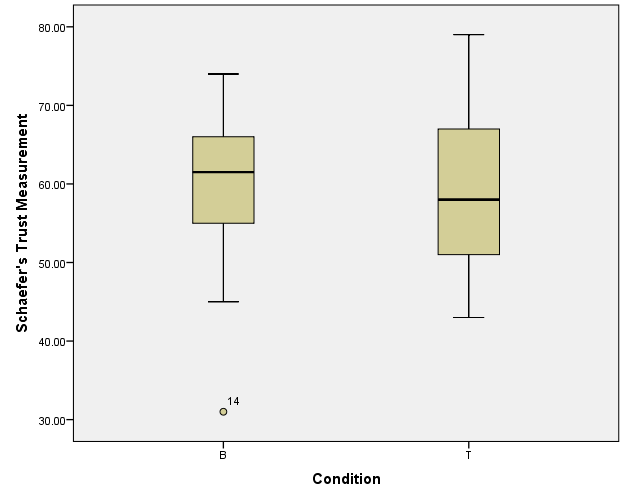
\includegraphics[width=0.6\textwidth]{graphs/Schaefer.png}
    \caption{Box-plot of Schaefer measurement results (Condition B Median: 61.5; Condition T Median: 58.0).}
    \label{fig:SchaeferMeasurementResults}
\end{figure}

\begin{table}[h]
    \centering
    \begin{tabular}{|l|l|l|}
        \hline
        \textbf{Descriptives}       &  \textbf{Condition B}     & \textbf{Condition T}  \\ \hline
        Mean                        &  59.05$\pm$2.32           & 59.47$\pm$2.64        \\ \hline
        Std. Deviation              &  10.38                    & 10.90                 \\ \hline
        Shapiro-Wilk Sig.           &  0.157                    & 0.622                 \\ \hline
        T-Test Mean Difference      &  -0.421                   & 0.421                 \\ \hline
        T-Test Sig.                 &  0.905                    & 0.906                 \\ \hline
    \end{tabular}
    \caption{Schaefer Measurements Descriptives.}
    \label{tbl:SchaeferMeasurementsDescriptives}
\end{table}

\textbf{Answer:} There were no significant differences between the means of Schaefer's Trust measurements in the 2 conditions.


\subsection*{Does the participant's Investment value in the scenario increase by the inclusion of the Action Suggestion module?}
Due to the distribution of the Investment value not being normal in condition B, as observed in the histograms in Figures \ref{fig:InvestmentConditionBHistogram} and \ref{fig:InvestmentConditionTHistogram}, we used Mann–Whitney U statistical test to determine if there is a significant difference between the results in each condition. Additionally, as the distribution shapes are quite different, we can only check through mean rank values. But with a significance p-value of $p=0.707$ in the Mann–Whitney U test we cannot conclude any significant difference in results between the conditions, evidenced further on the box-plot graph represented in Figure \ref{fig:InvestmentBoxPlot}.


\begin{figure}[h]
    \centering
    \begin{minipage}[b]{.45\textwidth}
        \centering
        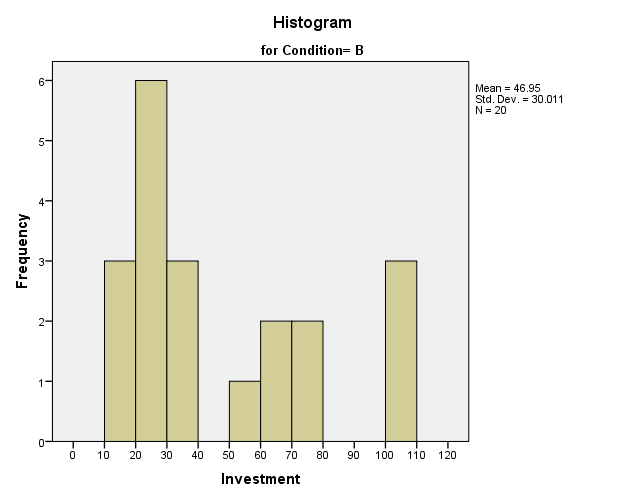
\includegraphics[width=\textwidth]{graphs/InvestmentHisto1.png}
        \caption{Investment values in Condition B Histogram}
        \label{fig:InvestmentConditionBHistogram}
    \end{minipage}
    \hfill
    \begin{minipage}[b]{.45\textwidth}
        \centering
        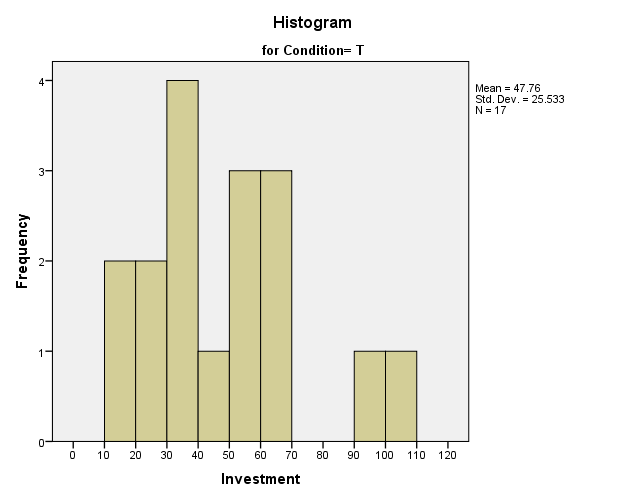
\includegraphics[width=\textwidth]{graphs/InvestmentHisto2.png}
        \caption{Investment values in Condition T Histogram}
        \label{fig:InvestmentConditionTHistogram}
    \end{minipage}
\end{figure}


\begin{figure}[hbt]
    \centering
    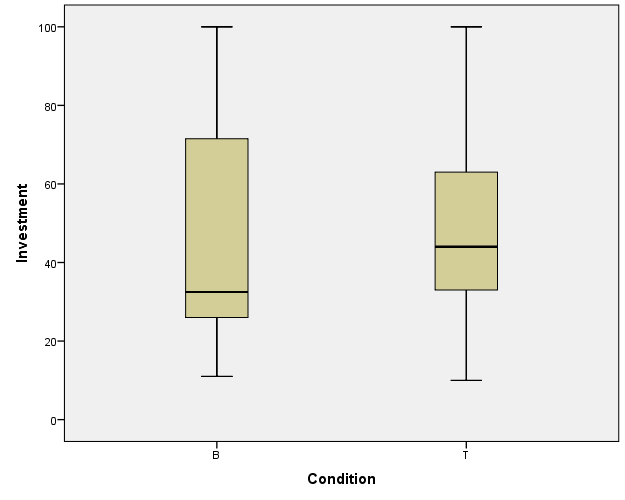
\includegraphics[width=0.5\textwidth]{graphs/InvestmentBoxPlot.png}
    \caption{Box-plot of scenario Investment measurement results (Condition B Median: 32.5; Condition T Median: 44.00).}
    \label{fig:InvestmentBoxPlot}
\end{figure}

\textbf{Answer}: There were no significant differences between the means of Investment value measurements in the 2 conditions.

\section{Results Discussion}
The study results show no statistical significant change in trust measurements between conditions B and T, leading to inconclusive results. But by observation of the box-plot graphs, seen in Figures \ref{fig:SchaeferMeasurementResults} and \ref{fig:InvestmentBoxPlot}, it seems that the Action Suggestion module had no effect on the participant's trust in the agent.
We believe that this results are due to the oversimplification of the implemented model, not only were the Actions just utterances, but these utterances were not properly verified as appropriate to increase Trust. Additionally, the participants commented that they could not pay that much attention to how the agent played, as the game required too much attention, so the games should be played non-concurrently, in order to give the participant opportunity to focus on how the agent plays the game.